\chapter{Fork --- オープンソースに貢献する}

\section{この章で学ぶこと}

この章では、GitHub上で最も魅力的な活動のひとつである「オープンソースソフトウェア（OSS）への貢献」について学びます。OSSとは、ソースコードが公開されており、誰でも自由に閲覧・利用・改変・再配布できるソフトウェアのことです。皆さんが普段使っているLinux、Python、VS Code、そしてGit自体もOSSです。

OSSへの貢献と聞くと、「自分にはまだ早い」「上級者がやることだ」と感じるかもしれません。しかし、実際にはタイポの修正やドキュメントの改善といった小さな貢献から始められますし、GitHubにはそのための仕組みが整っています。その中心にあるのが\textbf{Fork（フォーク）}という機能です。

この章を読み終えると、以下のことができるようになります。

\begin{itemize}
  \item Forkの仕組みと、通常のcloneとの違いを理解する
  \item OSSプロジェクトにPull Requestを送る一連の手順を実践できる
  \item upstreamリモートを設定し、Fork元のリポジトリと同期を保てる
  \item 貢献する前に確認すべきルールやマナーを理解する
  \item コード以外の貢献方法を知る
\end{itemize}

\section{Forkとは何か}

\subsection{他の人のリポジトリを自分のアカウントにコピーする}

Forkとは、GitHub上で他のユーザーやOrganizationが所有するリポジトリを、自分のGitHubアカウントの下にまるごとコピーする操作です。日本語では「分岐」や「派生」と訳されることもありますが、実際にはリポジトリの完全なコピーを自分のアカウントに作成する行為です。

なぜこのような仕組みが必要なのでしょうか。たとえば、あなたがあるOSSプロジェクトのバグを見つけて修正したいとします。しかし、そのリポジトリに対してあなたにはpush権限がありません。OSSプロジェクトは世界中の何千人もの開発者がアクセスしますが、全員にpush権限を与えてしまったら、コードの品質管理が不可能になってしまいます。

そこでForkの出番です。Forkを使えば、自分のアカウントにリポジトリのコピーを作り、そのコピーには自由にpushできます。修正が完了したら、元のリポジトリに対してPull Requestを送り、メンテナーにレビューしてもらうという流れになります。

\begin{lstlisting}[language={}]
元のリポジトリ (upstream)              あなたのFork (origin)
original-author/project    ──Fork──→    your-name/project
         ↑                                     │
         │                                     │ push（自由にできる）
         │                                     ↓
         └──────── Pull Request ───────────────┘
\end{lstlisting}

\subsection{cloneとの違い}

初学者がよく混同するのが、Forkとcloneの違いです。この2つは似ているようで、まったく異なる操作です。

\textbf{clone}は、リモートリポジトリをローカルマシンにダウンロードする操作です。\cmd{git clone}コマンドで実行し、結果としてローカルマシンにリポジトリのコピーが作られます。cloneしたリポジトリのリモート（origin）は、元のリポジトリを指しています。

\textbf{Fork}は、GitHubのサーバー上でリポジトリを自分のアカウントにコピーする操作です。これはGit自体の機能ではなく、GitHubが提供するWebサービスの機能です。Forkした結果、GitHub上に新しいリポジトリが作られ、そのリポジトリはあなたが自由に操作できます。

つまり、OSSに貢献する際は、まずGitHub上でForkし、次にForkしたリポジトリをローカルにcloneするという2段階の操作を行います。

\begin{tabular}{|l|l|l|l|}
\hline
\textbf{操作} & \textbf{実行場所} & \textbf{コピー先} & \textbf{push権限} \\
\hline
\textbf{clone} & ターミナル & ローカルマシン & 元のリポジトリの権限に依存 \\
\hline
\textbf{Fork} & GitHub Web / CLI & 自分のGitHubアカウント & 自分のForkには自由にpush可能 \\
\hline
\end{tabular}

Forkには、もうひとつ重要な特徴があります。GitHubはFork元のリポジトリとFork先のリポジトリの関連を記憶しています。これにより、Fork先からFork元へのPull Requestを簡単に作成できるのです。

\section{OSSへの貢献の全体像}

OSSプロジェクトに貢献する際の典型的なワークフローは、以下の6つのステップで構成されます。この流れは世界中のOSSプロジェクトで共通しており、一度覚えてしまえばどのプロジェクトにも応用できます。

\begin{lstlisting}[language={}]
┌─────────────────────────────────────────────────────────┐
│                   OSSコントリビューションの流れ              │
├─────────────────────────────────────────────────────────┤
│                                                         │
│  ① Fork       GitHub上でリポジトリをコピー                │
│      ↓                                                  │
│  ② Clone      Forkをローカルにダウンロード                │
│      ↓                                                  │
│  ③ Branch     作業用ブランチを作成                        │
│      ↓                                                  │
│  ④ Commit     変更を加えてコミット                        │
│      ↓                                                  │
│  ⑤ Push       自分のForkにプッシュ                       │
│      ↓                                                  │
│  ⑥ PR         元のリポジトリにPull Requestを送信          │
│                                                         │
└─────────────────────────────────────────────────────────┘
\end{lstlisting}

この流れを、図書館の本に例えてみましょう。図書館（元のリポジトリ）の本に誤植を見つけたとします。図書館の本に直接ペンで書き込むわけにはいきません。そこで、本をコピーして（Fork）、自分の机に持ち帰り（clone）、修正案を書いたメモを挟み（branch + commit）、コピーに修正を反映させ（push）、図書館に「ここを直してはどうでしょうか」と提案書を送ります（Pull Request）。図書館員（メンテナー）がその提案を確認して妥当だと判断すれば、本が修正されます。

このワークフローの優れている点は、元のリポジトリに影響を与えることなく安全に作業でき、かつ正式なレビュープロセスを経て貢献を反映できるところにあります。

\section{実践手順}

ここからは、実際のコマンドを使って貢献の手順を一つひとつ見ていきましょう。例として、\cmd{original-author/project}というリポジトリに貢献する場面を想定します。

\subsection{ステップ1: Forkする}

Forkの方法は2通りあります。GitHub CLIを使う方法と、WebブラウザのUIを使う方法です。

GitHub CLIの\cmd{gh repo fork}コマンドを使うと、Forkとcloneを一度に行えます。\cmd{--clone}フラグを付けると、Forkした直後にローカルへのcloneも自動的に行われるため、初心者にはこちらがおすすめです。

\begin{lstlisting}[language=bash]
# CLIでFork（cloneも同時に行う）
gh repo fork original-author/project --clone
cd project
\end{lstlisting}

Webブラウザを使う場合は、貢献したいリポジトリのページを開き、右上にある「Fork」ボタンをクリックします。Forkが完了すると、\cmd{your-name/project}というリポジトリが自分のアカウントに作成されます。その後、手動でcloneします。

\begin{lstlisting}[language=bash]
# Web UIでForkした後、自分のForkをクローン
git clone git@github.com:your-name/project.git
cd project
\end{lstlisting}

\begin{figure}[htbp]
\centering
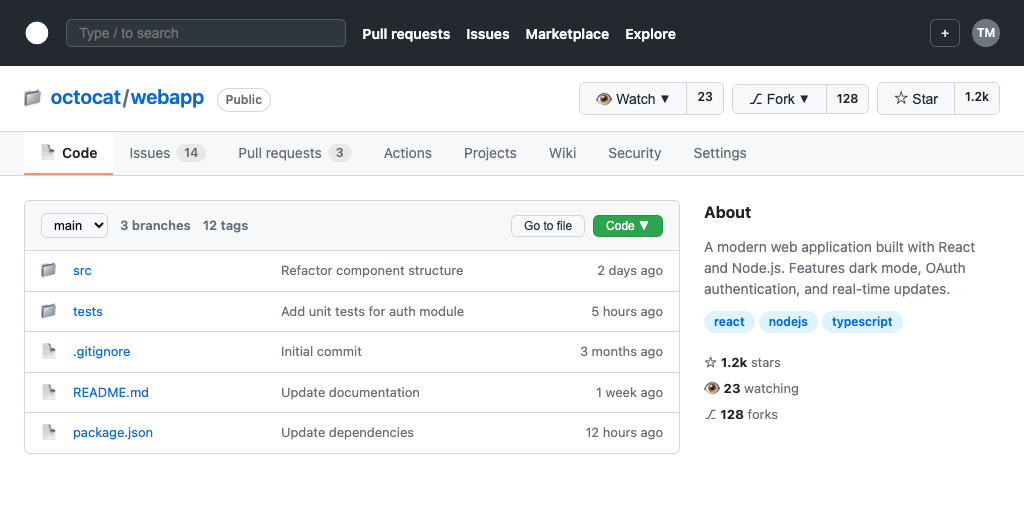
\includegraphics[width=0.95\textwidth]{images/fork-button.png}
\caption{リポジトリページ右上のForkボタン}
\end{figure}

\subsection{ステップ2: upstreamリモートを設定する}

cloneした直後、リモートには\cmd{origin}（自分のFork）だけが登録されています。しかし、Fork元のリポジトリ（upstream）も登録しておく必要があります。なぜなら、Fork元のリポジトリは日々更新されており、自分のForkをその最新の状態に同期させる必要があるからです。

\cmd{upstream}という名前はGitの慣習で、Fork元のリポジトリを指す際に広く使われています。この名前を使うことで、他の開発者があなたのコマンド履歴を見たときにも意図が伝わりやすくなります。

\begin{lstlisting}[language=bash]
# Fork元をupstreamとして登録
git remote add upstream git@github.com:original-author/project.git

# リモートの設定を確認
git remote -v
# origin    git@github.com:your-name/project.git (fetch)
# origin    git@github.com:your-name/project.git (push)
# upstream  git@github.com:original-author/project.git (fetch)
# upstream  git@github.com:original-author/project.git (push)
\end{lstlisting}

\cmd{git remote -v}の出力を見て、\cmd{origin}が自分のFork、\cmd{upstream}がFork元のリポジトリを指していることを確認しましょう。もしURLが間違っていた場合は、\cmd{git remote set-url upstream 正しいURL}で修正できます。

なお、\cmd{gh repo fork --clone}でForkとcloneを同時に行った場合は、upstreamの設定も自動的に行われます。

\subsection{ステップ3: Fork元の最新の状態と同期する}

OSSプロジェクトでは、あなたがForkしてから作業を始めるまでの間にも、他の貢献者によってコードが更新されている可能性があります。古い状態のコードに対して作業を行うと、最終的にPull Requestを送る際にコンフリクト（衝突）が発生しやすくなります。

そのため、作業を始める前にFork元の最新の状態を取り込む習慣をつけましょう。この操作は、長期間にわたって作業する場合は定期的に行います。

\begin{lstlisting}[language=bash]
# upstreamの最新を取得
git fetch upstream

# mainブランチに切り替え
git switch main

# upstreamのmainブランチの内容をマージ
git merge upstream/main

# 同期した内容を自分のFork（origin）にもプッシュ
git push origin main
\end{lstlisting}

\cmd{git fetch upstream}はupstreamの情報をダウンロードするだけで、ローカルのファイルには変更を加えません。その後の\cmd{git merge upstream/main}で、ダウンロードした内容を実際にローカルのmainブランチに反映します。最後に\cmd{git push origin main}で、自分のFork上のmainブランチも最新にしておきます。

\subsection{ステップ4: ブランチを作成して作業する}

貢献の作業は、必ず専用のブランチで行いましょう。mainブランチで直接作業してしまうと、同期の際に問題が起きやすくなります。ブランチ名は、変更の内容が分かるような名前を付けます。多くのOSSプロジェクトでは、\cmd{fix/}、\cmd{feat/}、\cmd{docs/}といったプレフィックスを使う慣習があります。

\begin{lstlisting}[language=bash]
# 作業ブランチを作成して切り替え
git switch -c fix/typo-in-readme

# ファイルを編集する（ここでは例としてREADME.mdのタイポ修正）
# ... エディタで編集 ...

# 変更をステージングしてコミット
git add README.md
git commit -m "fix: Fix typo in installation section"

# 自分のForkにプッシュ
git push -u origin fix/typo-in-readme
\end{lstlisting}

コミットメッセージについても、プロジェクトの規約に従うことが大切です。多くのプロジェクトではConventional Commitsのようなルールを採用しています。CONTRIBUTING.mdに記載がある場合は、必ずそれに従いましょう。

\subsection{ステップ5: Pull Requestを送る}

変更をForkにプッシュしたら、いよいよ元のリポジトリに対してPull Requestを送ります。CLIからもWebブラウザからも作成できます。

\begin{lstlisting}[language=bash]
# CLIでPRを作成（Fork元のリポジトリを指定する）
gh pr create --repo original-author/project \
  --title "fix: Fix typo in README" \
  --body "READMEのインストール手順にあるタイポを修正しました。

## 変更内容
- 「instlation」を「installation」に修正

## テスト
- ドキュメントの変更のみのため、動作テストは不要です。"
\end{lstlisting}

Webブラウザを使う場合は、自分のForkリポジトリのページを開くと、最近プッシュしたブランチの通知バーが表示されます。そこから「Compare \& pull request」をクリックするか、「Contribute」ボタンから「Open pull request」を選択します。

\screenshot{ForkリポジトリからPull Requestを作成する画面}

Pull Requestの説明文（body）は丁寧に書きましょう。メンテナーはあなたの変更の意図を理解する必要があります。何を変更したのか、なぜ変更が必要なのか、どのようにテストしたのかを明記すると、レビューがスムーズに進みます。

\subsection{ステップ6: レビュー対応}

Pull Requestを送った後、プロジェクトのメンテナーがコードをレビューしてくれます。レビューでは修正のリクエストが来ることがよくあります。これは自然なプロセスであり、否定されているわけではありません。むしろ、プロジェクトの品質を保つための重要な工程です。

修正が必要な場合は、同じブランチで作業を続けます。新しいコミットをプッシュすると、Pull Requestに自動的に反映されます。

\begin{lstlisting}[language=bash]
# 作業ブランチに切り替え（すでにいる場合は不要）
git switch fix/typo-in-readme

# レビューのフィードバックに基づいて修正
# ... エディタで修正 ...

# 修正をコミットしてプッシュ
git add .
git commit -m "fix: Address review feedback - update wording"
git push
# → Pull Requestに自動的に反映される
\end{lstlisting}

レビュアーのコメントにはGitHub上で返信し、修正した箇所については「修正しました」と報告しましょう。すべての指摘に対応したら、レビュアーに再レビューをリクエストできます。

\section{貢献の前に確認すべきこと}

OSSプロジェクトに貢献する際は、コードを書き始める前に確認すべき重要な事項がいくつかあります。これらを事前に確認しておくことで、無駄な作業を避け、プロジェクトのメンテナーとのコミュニケーションを円滑に進められます。

\subsection{CONTRIBUTING.md}

多くのOSSプロジェクトには、\cmd{CONTRIBUTING.md}というファイルが置かれています。このファイルには、貢献の手順、コーディング規約、コミットメッセージのフォーマット、テストの方法など、そのプロジェクト独自のルールが記載されています。

\begin{lstlisting}[language=bash]
# CONTRIBUTING.mdの内容を確認する
cat CONTRIBUTING.md
\end{lstlisting}

たとえば、あるプロジェクトでは「Pull Requestを送る前に必ずIssueを立ててください」というルールがあるかもしれません。別のプロジェクトでは「コミットメッセージはConventional Commitsに従ってください」と指定されているかもしれません。こうしたルールを無視してPull Requestを送ると、レビューの前にフォーマットの修正を求められてしまいます。

\subsection{Code of Conduct（行動規範）}

\cmd{CODE\_OF\_CONDUCT.md}は、コミュニティでの振る舞いに関するルールを定めた文書です。差別的な発言の禁止、建設的なコミュニケーションの奨励、ハラスメントの禁止などが記載されています。多くのプロジェクトがContributor Covenantをベースにした行動規範を採用しています。

行動規範は堅苦しいものに感じるかもしれませんが、その本質は「お互いを尊重し、安心して参加できるコミュニティを作ろう」ということです。コメントやレビューでは常に敬意を持った言葉遣いを心がけましょう。

\subsection{good first issue を探す}

OSSプロジェクトに初めて貢献する場合、何から手を付ければよいか分からないことがあります。そんなときに役立つのが、\cmd{good first issue}ラベルです。このラベルが付いたIssueは、プロジェクトのメンテナーが「初めての貢献者でも取り組みやすい」と判断したものです。

\begin{lstlisting}[language=bash]
# good first issueラベルが付いたIssueを検索
gh issue list --repo original-author/project --label "good first issue"
\end{lstlisting}

\begin{figure}[htbp]
\centering
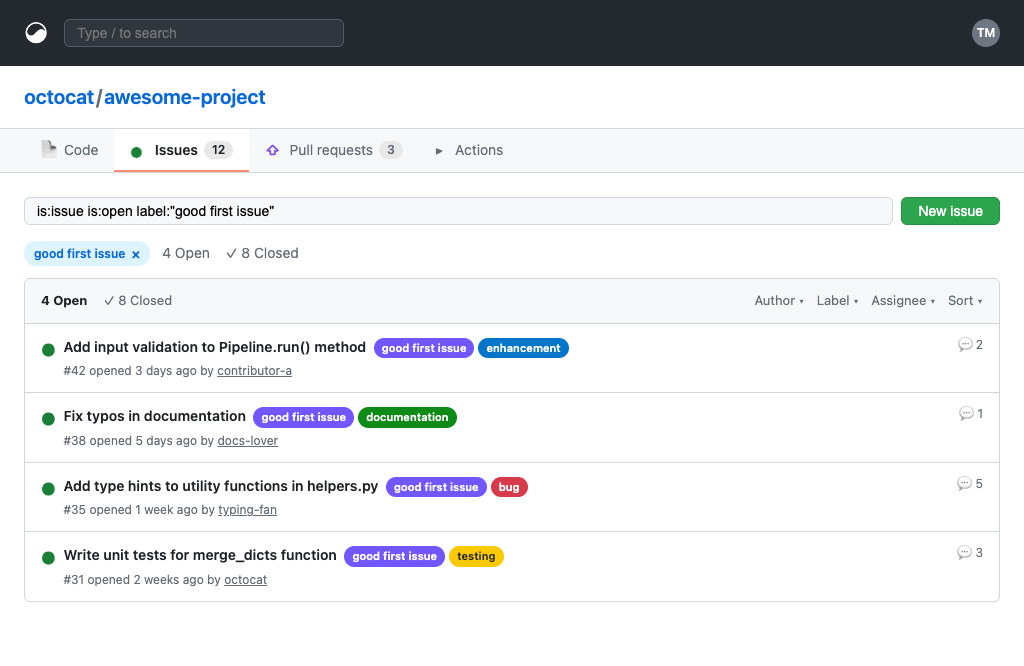
\includegraphics[width=0.95\textwidth]{images/good-first-issue.png}
\caption{good first issueラベルが付いたIssueの一覧}
\end{figure}

作業を始める前に、そのIssueにコメントを残して「この課題に取り組みたい」と宣言するのがマナーです。これにより、他の貢献者と作業が重複することを防げます。もしIssueにすでに誰かがアサインされている場合は、別のIssueを探しましょう。

\subsection{ライセンスの確認}

プロジェクトのライセンス（\cmd{LICENSE}ファイル）も確認しておきましょう。あなたが書いたコードはそのプロジェクトのライセンスの下で公開されます。一部のプロジェクトでは、CLA（Contributor License Agreement）への署名を求められることがあります。CLAとは、あなたが貢献するコードの権利関係を明確にするための同意書です。

\section{コード以外のコントリビューション}

OSSへの貢献というと、まずコードを書くことを思い浮かべるかもしれません。しかし、実際にはコード以外にも非常に多くの貢献の形があります。むしろ、コード以外の貢献が足りていないプロジェクトは数多くあり、そうした領域での貢献はメンテナーにとても感謝されます。

\subsection{ドキュメントの改善}

ドキュメントの誤字脱字の修正、分かりにくい説明の書き直し、インストール手順の更新など、ドキュメントに関する貢献は常に歓迎されます。特に、初心者としてドキュメントを読んだときに「ここが分かりにくかった」という気づきは、それ自体が貴重なフィードバックです。経験豊富な開発者は自分の知識を前提にしてしまいがちなので、新鮮な目で見た改善提案は大きな価値があります。

\subsection{翻訳}

国際的なプロジェクトでは、ドキュメントやUIの翻訳が求められることがあります。英語から日本語への翻訳は、日本語話者にとって取り組みやすい貢献のひとつです。プロジェクトによっては、Crowdinなどの翻訳プラットフォームを使っている場合もあります。

\subsection{Issue報告}

バグを発見した際に、再現手順を明確に記載したバグレポートを提出することも立派な貢献です。良いバグレポートには、使用環境（OS、ブラウザ、バージョンなど）、期待される動作、実際の動作、再現手順が含まれています。メンテナーが問題を素早く理解し修正できるよう、できるだけ具体的に書きましょう。

機能の提案（Feature Request）も同様に価値のある貢献です。ただし、提案の前にIssueの一覧を検索して、同じ提案がすでにないか確認しましょう。

\subsection{レビュー}

他の貢献者が送ったPull Requestをレビューすることも、プロジェクトへの大きな貢献になります。メンテナーのレビュー負担を軽減できるだけでなく、自分自身のコードリーディング力も向上します。

\subsection{デザイン}

UIやUXの改善提案、アイコンの作成、Webサイトのデザインなど、デザインの専門知識を活かした貢献も重要です。多くのOSSプロジェクトは開発者が中心であるため、デザイン面での貢献は特に不足しがちです。

\begin{tabular}{|l|l|l|}
\hline
\textbf{貢献の種類} & \textbf{具体例} & \textbf{必要なスキル} \\
\hline
\textbf{コード} & バグ修正、新機能の実装 & プログラミング \\
\hline
\textbf{ドキュメント} & README改善、チュートリアル作成 & 文章力 \\
\hline
\textbf{翻訳} & UIやドキュメントの多言語化 & 語学力 \\
\hline
\textbf{Issue報告} & バグレポート、機能提案 & 丁寧な記述力 \\
\hline
\textbf{レビュー} & Pull Requestのコードレビュー & コードリーディング力 \\
\hline
\textbf{テスト} & テストケースの追加、手動テスト & テスト設計力 \\
\hline
\textbf{デザイン} & UI/UXの改善、アイコン作成 & デザインスキル \\
\hline
\end{tabular}

\section{まとめ}

この章では、Forkの仕組みとOSSへの貢献の流れについて学びました。重要なポイントを振り返りましょう。

\begin{itemize}
  \item \textbf{Fork}は、GitHub上で他のリポジトリを自分のアカウントにコピーする操作であり、cloneとは異なるGitHub固有の機能である
  \item OSSへの貢献は、\textbf{Fork → clone → branch → commit → push → Pull Request}という一連の流れで行う
  \item \textbf{upstream}リモートを設定し、Fork元のリポジトリと定期的に同期することで、コンフリクトを防ぐ
  \item 貢献を始める前に、\textbf{CONTRIBUTING.md}、\textbf{Code of Conduct}、\textbf{ライセンス}を確認する
  \item \textbf{good first issue}ラベルの付いたIssueは、初心者にとって最適な出発点となる
  \item コード以外にも、\textbf{ドキュメント、翻訳、Issue報告、レビュー、デザイン}など多様な貢献方法がある
\end{itemize}

OSSへの貢献は、自分のスキルを向上させると同時に、世界中の開発者が使うソフトウェアをより良くする素晴らしい活動です。最初の一歩は小さくても構いません。まずは好きなプロジェクトの\cmd{good first issue}を覗いてみるところから始めてみてください。
